\subsection{External Interface Requirements}
\subsubsection{User interfaces}
In the design document there will be the specific application UI created after the process (UX) of defining how users interact with SafeStreets.
The following mocks describe only the generic application screen design:

	\begin{figure}[H]
		\centering
		\begin{minipage}[b]{0.40\textwidth}
			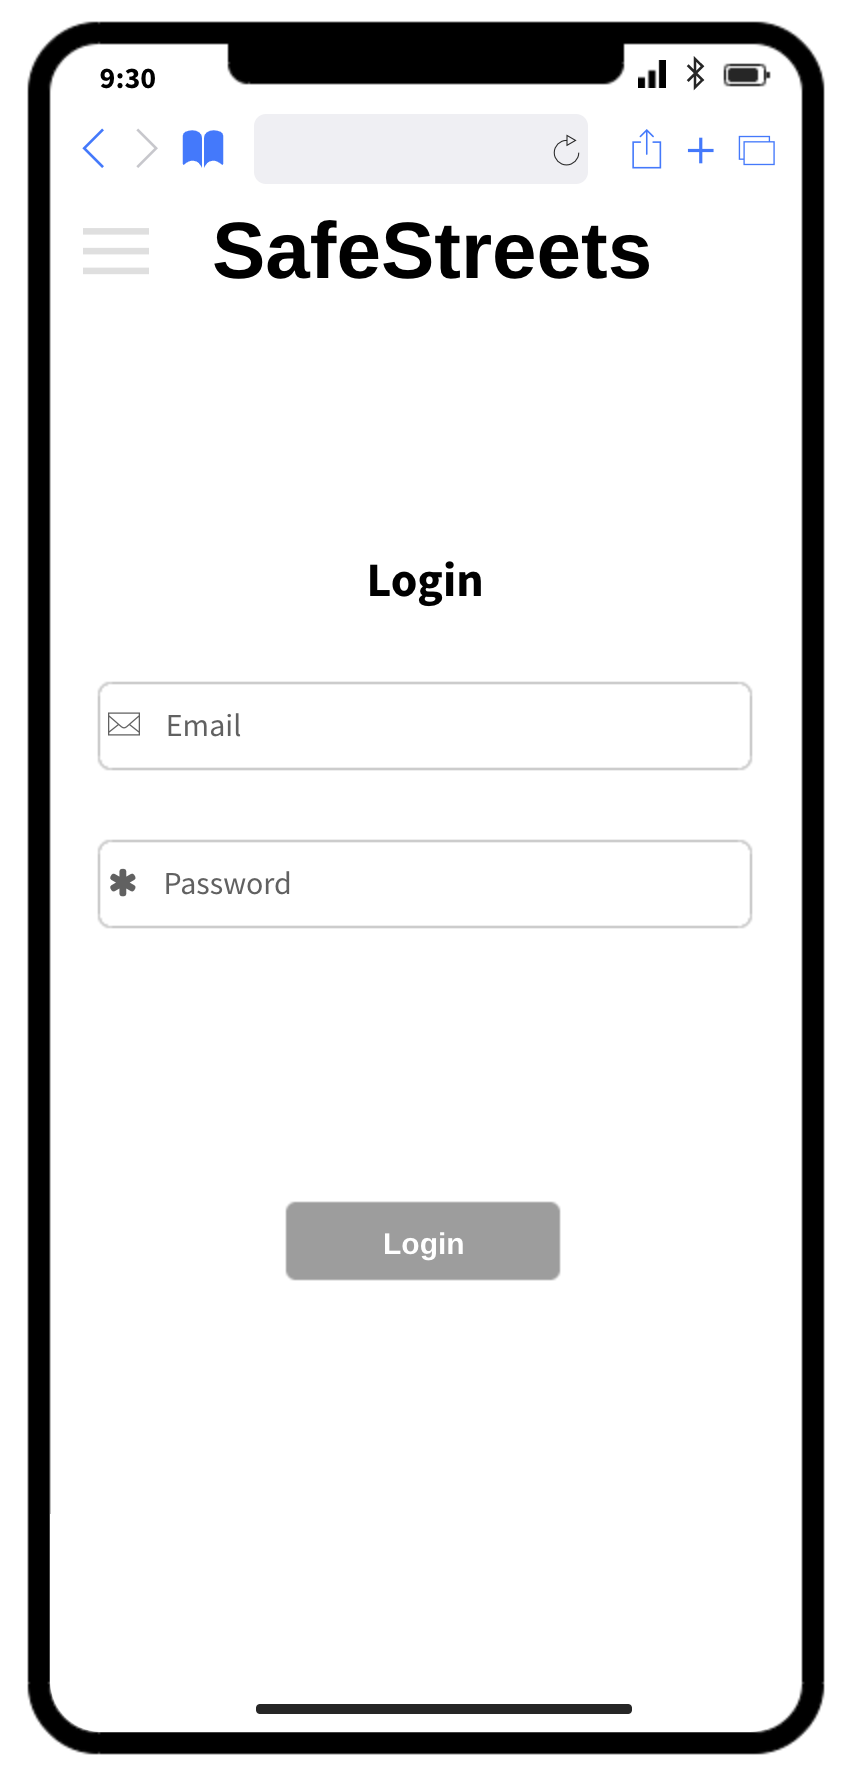
\includegraphics[width=\textwidth]{Images/rasd-mocks/login.png}
			\caption{Login form}
		\end{minipage}
		\hfill
		\begin{minipage}[b]{0.40\textwidth}
			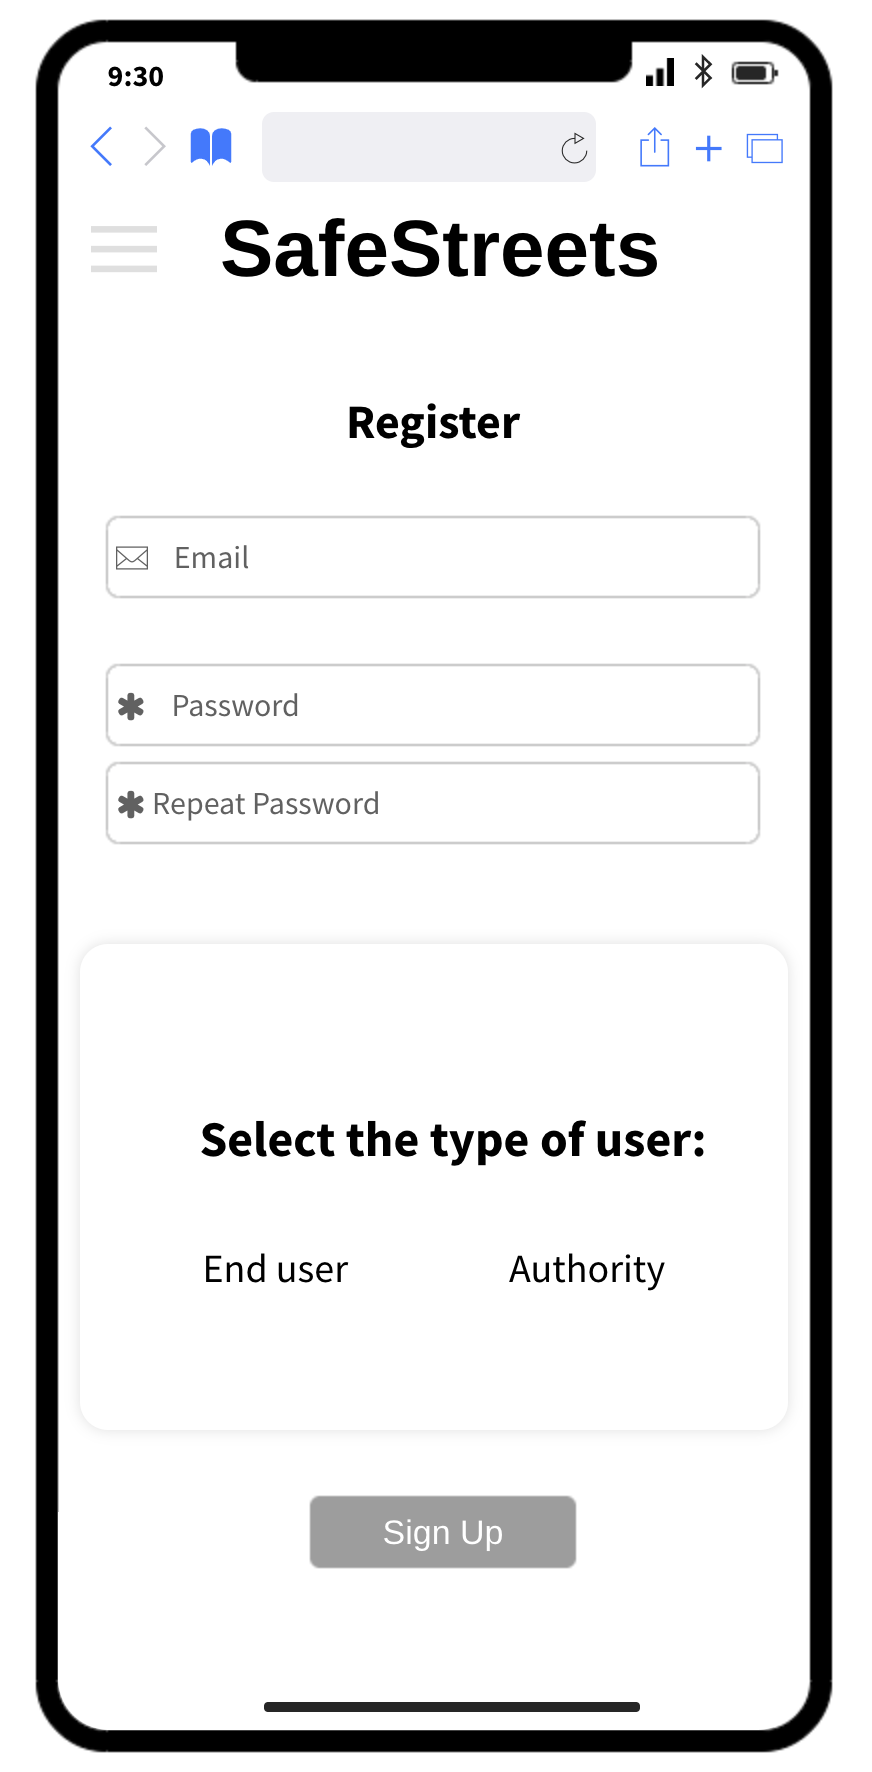
\includegraphics[width=\textwidth]{Images/rasd-mocks/registration.png}
			\caption{Registration form}
		\end{minipage}
	\end{figure}

\newpage
	
		\begin{figure}[H]
		\centering
		\begin{minipage}[b]{0.40\textwidth}
			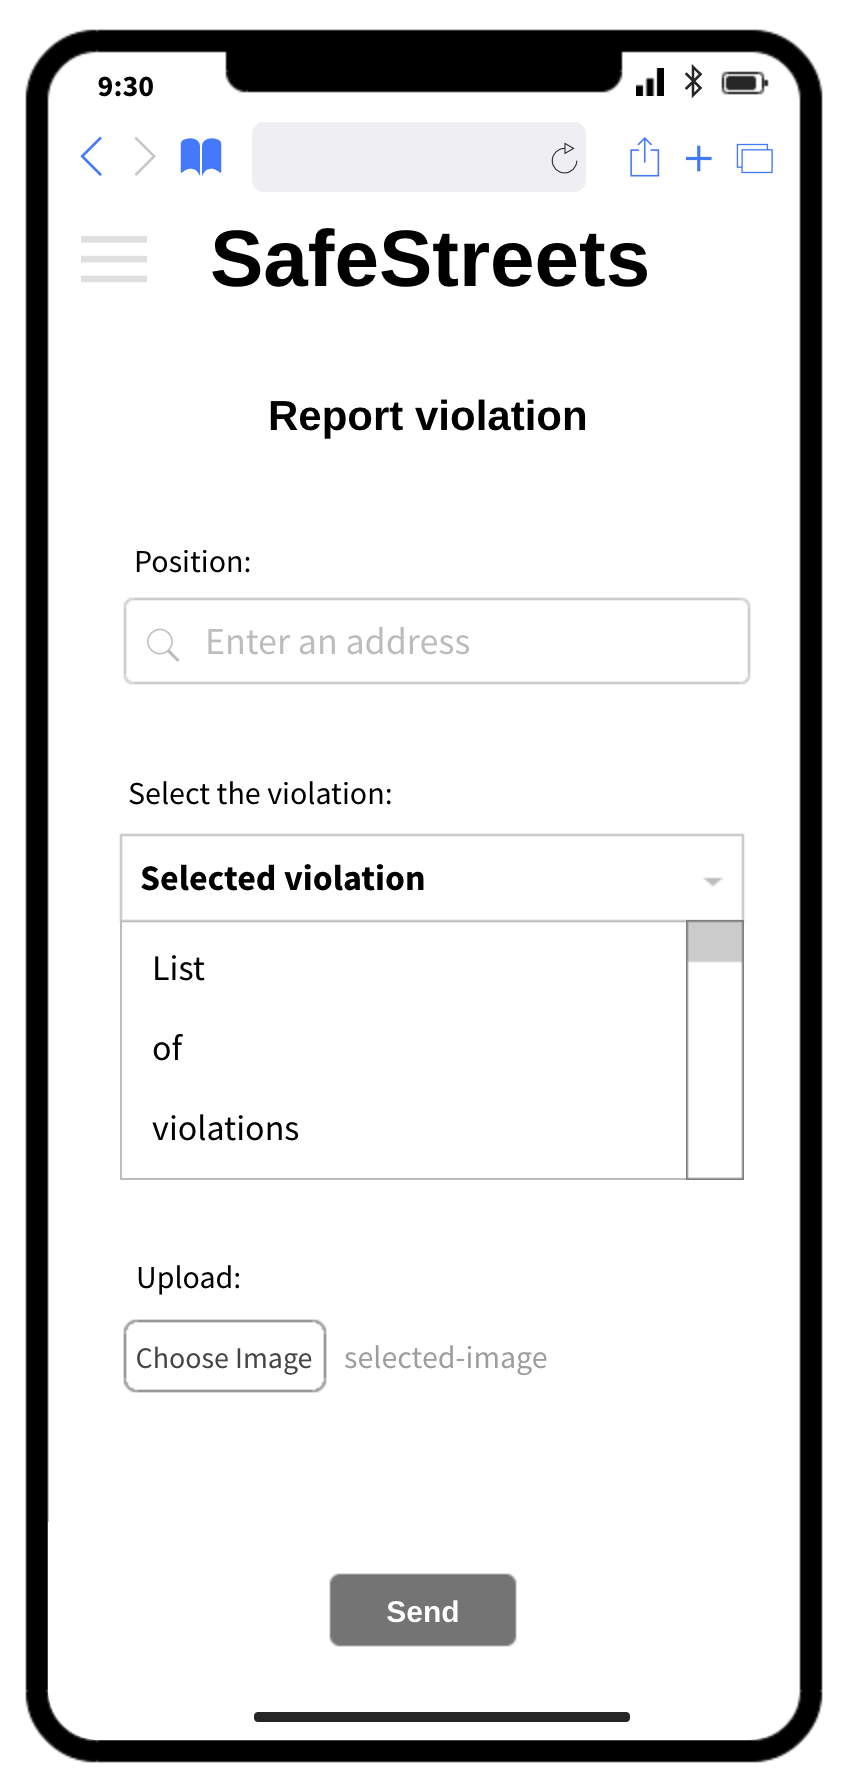
\includegraphics[width=\textwidth]{Images/rasd-mocks/report.png}
			\caption{User send violation report}
		\end{minipage}
		\hfill
		\begin{minipage}[b]{0.40\textwidth}
			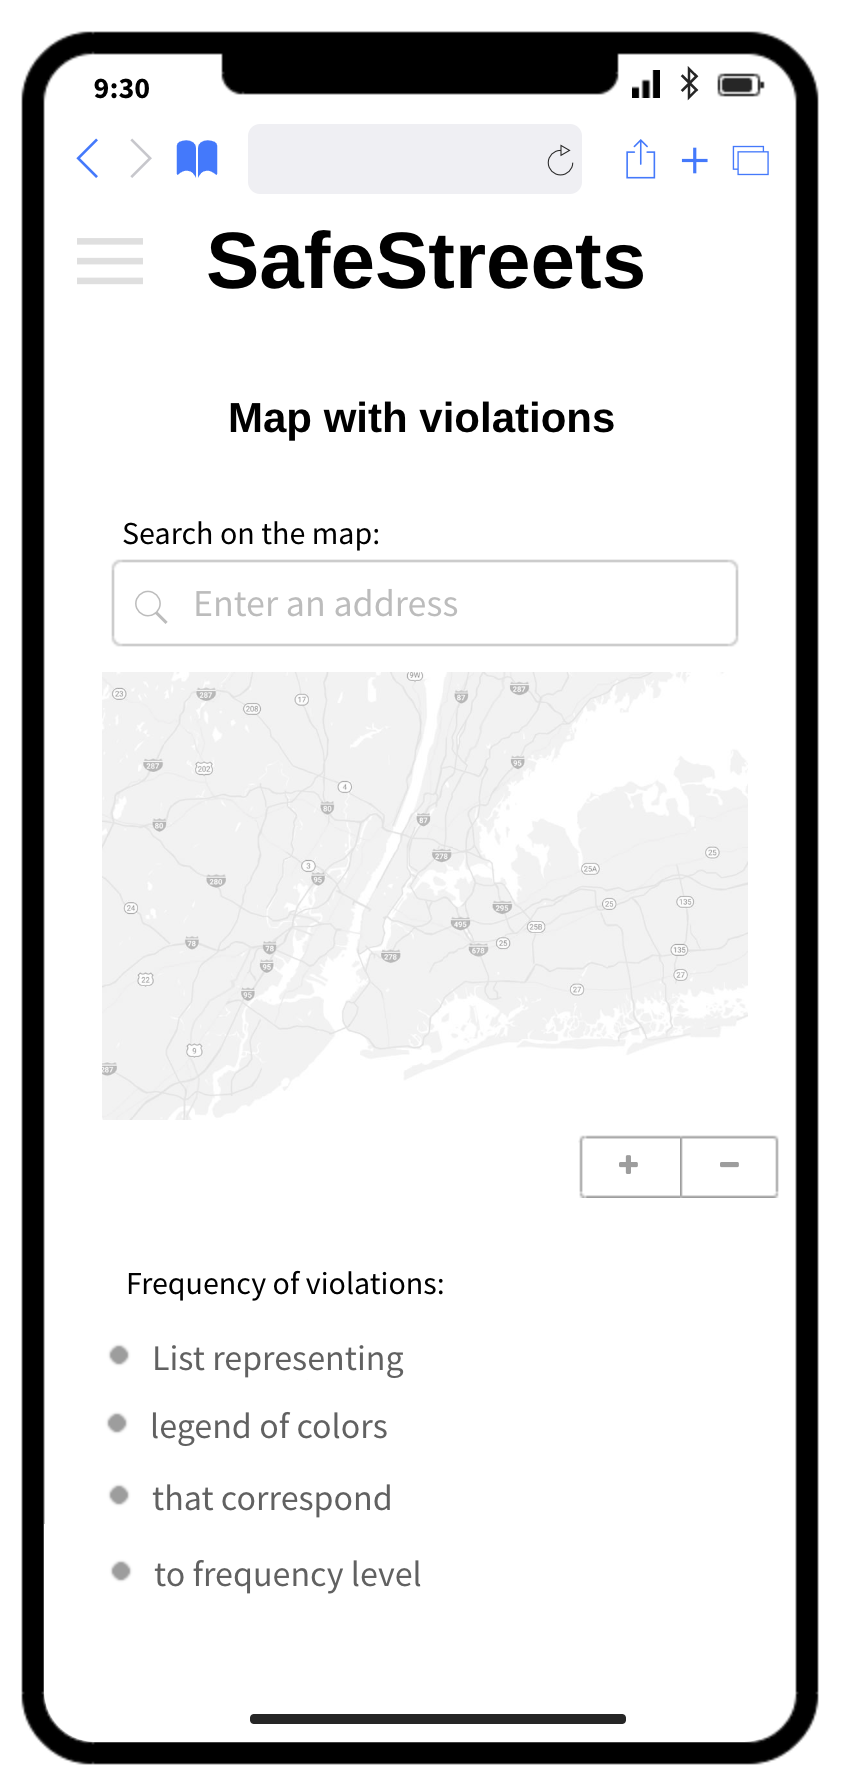
\includegraphics[width=\textwidth]{Images/rasd-mocks/violationsMap.png}
			\caption{Map showing violations}
		\end{minipage}
	\end{figure}

	\begin{figure}[H]
	\centering
	\begin{minipage}[b]{0.40\textwidth}
		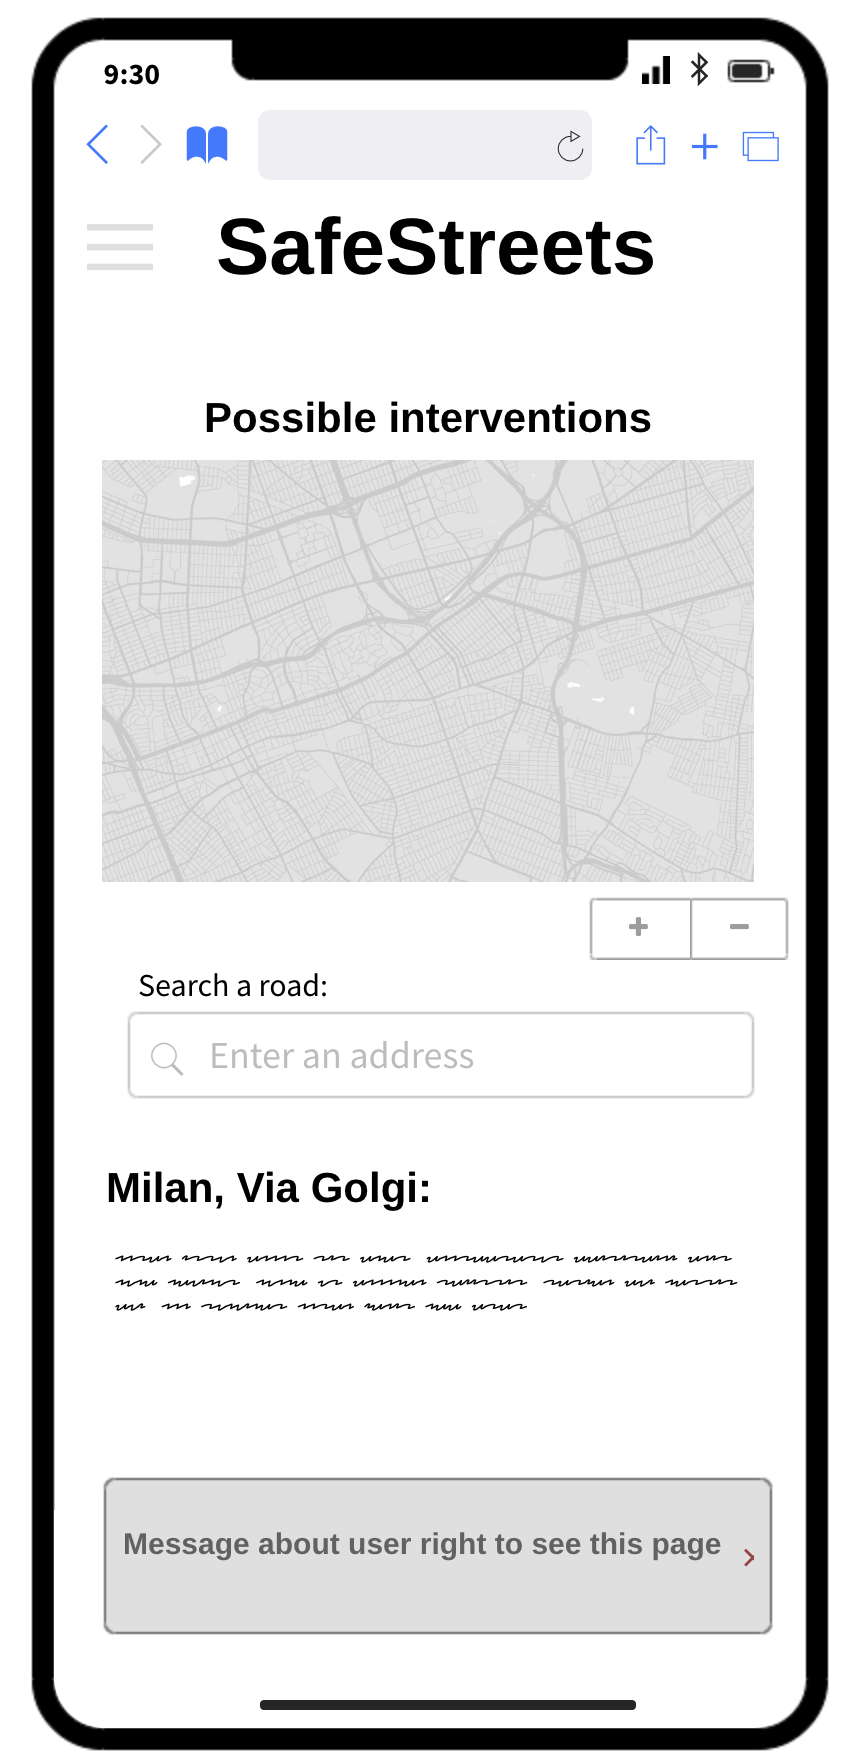
\includegraphics[width=\textwidth]{Images/rasd-mocks/interventions.png}
		\caption{Suggestion for possible interventions}
	\end{minipage}
	\hfill
	\begin{minipage}[b]{0.40\textwidth}
		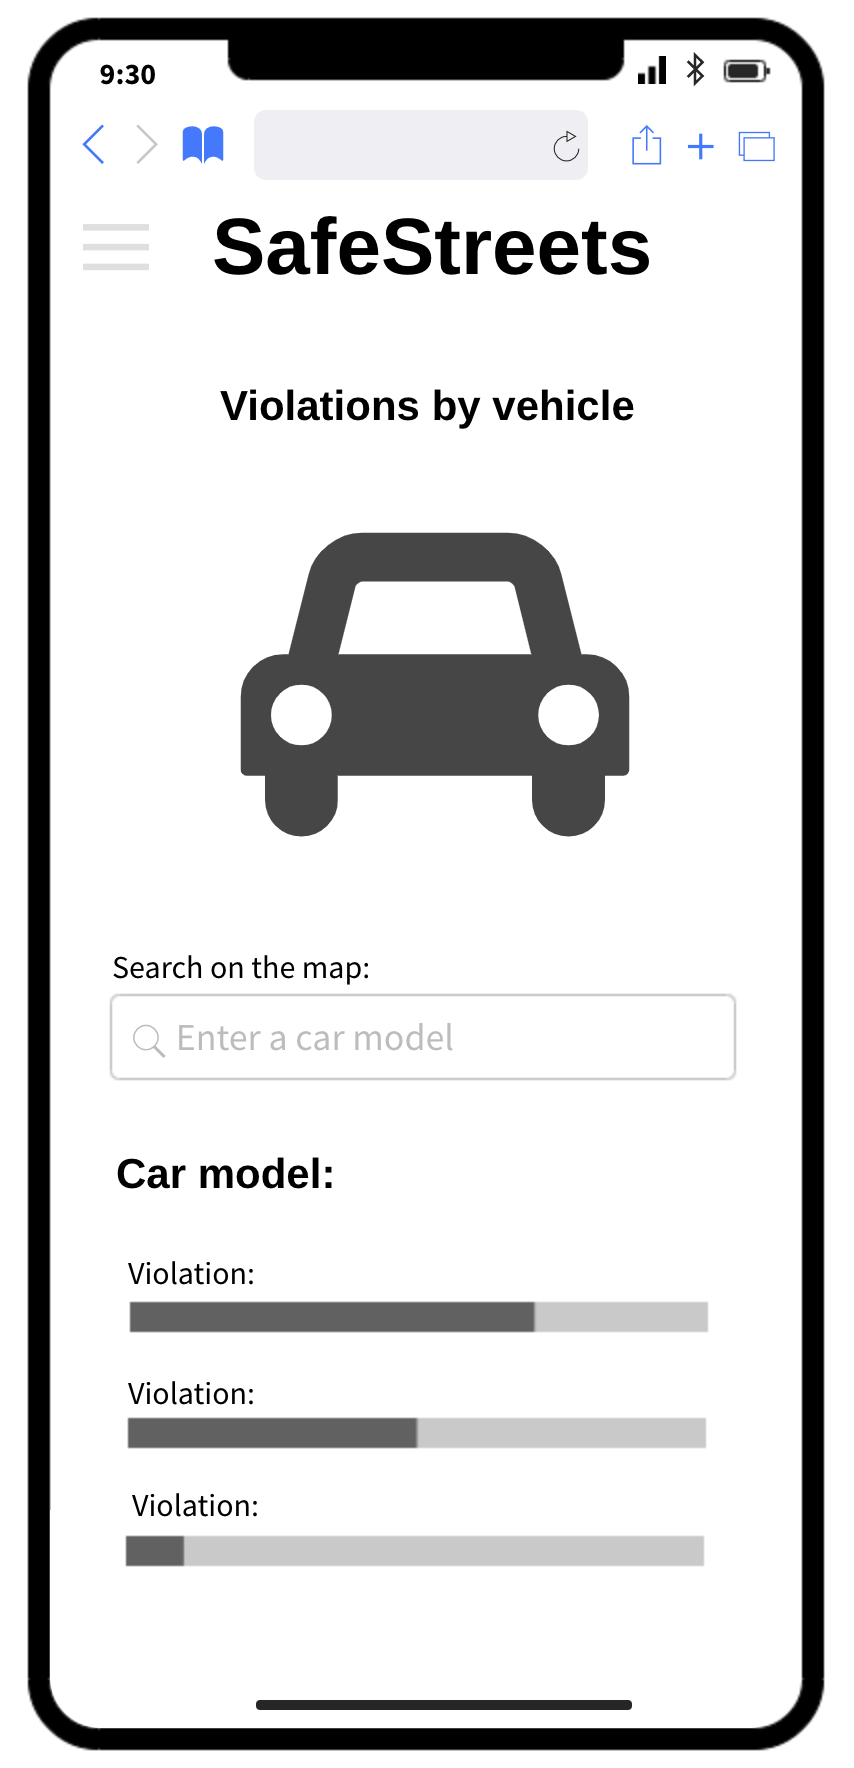
\includegraphics[width=\textwidth]{Images/rasd-mocks/vehicle.png}
		\caption{Violations by vehicle}
	\end{minipage}
\end{figure}

\subsubsection{Hardware interfaces}


\subsubsection{Software interfaces}
The system functionalities are provided with the usage of some external web services:

\paragraph{Google Maps}
Google Maps library is used in the page that shows the map.
Furthermore, Google Maps APIs are used to transform addresses in coordinates and vice versa.


\paragraph{Vehicle model identification}
Using an external web service, SafeStreets is able to retrieve information about the vehicles from the license plate number.
This data will be show in statistics about violations by vehicles.

\paragraph{IndicePA}
The \textit{CUU (Codice Univoco Ufficio)} verification is made by an external web service provided by \textit{IndicePA}. The code is required during the authorities registration to ensure their identity.
The external API are exposed only for authorities application and the implementation details will be shown in the design document (DD).


\subsubsection{Communication interfaces}
Any communication functionality takes place via internet with HTTPS to allow protection and privacy.

This protocol will be used for both access to the web-application and REST communication.

\subsection{Design constraints}
\subsubsection{Standards compliance}
Part of the information collected by SafeStreets (e.g. license plate) are sensitive. For this reason the project is subject to the \textit{General Data Protection Regulation (GDPR)}. 

One of the technique used by the system to protect these important information is the creation of different type of users. 

For example normal account can only send information and see general information.
While authorities have a different account that is able to access to the collected and generated data in details.

\subsubsection{Hardware limitations}
The application is based on retrieving data from the pictures sent by the user. 

Obviously the camera of the devices is a crucial aspect to consider during the design process. For this reason a minimum resolution of the sensor is required to install the application.

The identification of this value will be done during design phase and will be written in the design document (DD).

An other constraint is generated by the precision of the GPS sensor of the device, since the impact is smaller than the image resolution, the requirement is not so strict. 

\subsubsection{Any other constraint}
SafeStreets works with violations and traffic tickets so it has to deal with laws and regulations; for this aspect see the specific domain assumption.

Furthermore we have to consider the possible improper use of the platform. To prevent it, SafeStreets does specific controls on images and it is able to detect manipulations or repeated pictures of the same violations. 

The implementation of this part will be done with some external algorithm and will be detailed in the design document (DD).

\subsection{Functional requirements}
\subsubsection{Definition of use case diagram}
The use case diagrams provide a vision of the uses that can be done with the platform. 

They show the relationship between the actors and the use that every actor made with the software to reach the goals.

\subsubsection{Scenario 1}
Paul wants to sign up to SafeStreets platform. He has to insert his personal data (name, surname, place, mail and so forth). Then he will receive a confirm mail and can use the platform.

\subsubsection{Scenario 2}
Bob is coming back to his car when he notice that someone double parked and he can’t go out from the parking. 

He logs in into the SafeStreets and he takes a picture of the car to report it to the platform which will analyzes the report.

\subsubsection{Scenario 3}
Luke is walking on the sidewalk when he see that a man is parking on a park reserved for disable.
Luke takes a picture of the car and report it to the SafeStreets platform which analyzes the report,

\subsubsection{Scenario 4}
Mark has submitted a report to the platform, and he wants to check if it has been accepted or declined.
He logs in into the app, he goes to his reserved area and next to his report there is the status of message sent.

\subsubsection{Scenario 5}
An accidents in via Anzani occurs, the municipality system records the information about.
SafeStreets is able to retrieve a portion of these data and cross it with violations information, in order to generate statistics.

\subsubsection{Scenario 6}
The local authority wants to check which are the streets with more violations. They log in into the platform and access to their personal area where they can check the streets status.
 
\subsubsection{Scenario 7}
The local authority wants to check which are the vehicles with more violations. They log in into the platform and access to their personal area where they can check the cars that have the most reports assigned.

\subsubsection{Scenario 8}
The system receives pictures from the users and have to check if they are reliable. It runs an algorithm that can detect if the photo is real or it has been manipulated. In the first case, the report will be stored and be used by authorities. In the second case the report will be discarded.


\subsection{Description of use case scenarios}
\subsubsection{Description scenario 1}


\begin{center}
	\begin{tabular}{ | l | p{6cm} | } 
		\hline
		ACTORS & Visitors  \\ 
		\hline
		GOALS & Sign up  \\ 
		\hline
		INPUT CONDITION & Personal data (name, surname, mail, telephone number, place where he lives, car license plate etc.)  \\ 
		\hline
		EVENTS FLOW & The user from the home page clicks on sign up. He inserts all of his information and if it is all correct he will recive an email of confirm.  \\ 
		\hline
		OUTPUT CONDITION & The user can now log in and use all the function that the user can do on the platform.  \\ 
		\hline
		EXCEPTIONS & Data incorrect, user already exists, mail already exists. All of this exceptions will be notified instantly to the user. \\ 
		\hline
	\end{tabular}
\end{center}

\subsubsection{Description scenario 2}

\begin{center}
	\begin{tabular}{ | l | p{6cm} | } 
		\hline
		ACTORS & User  \\ 
		\hline
		GOALS & Report a violation  \\ 
		\hline
		INPUT CONDITION & Type of violation (double row park), name of the street,  \\ 
		\hline
		EVENTS FLOW & The user take a picture of the car that has done the violation. The system use an algorithm to read the car license plate and then store all the informations once it is established that the photo isn't fake.  \\ 
		\hline
		OUTPUT CONDITION & The violation has been stored with all the data, it will be generated a traffic ticket, and the local authority can decide to highlight who has made the violation or the street. \\ 
		\hline
		EXCEPTIONS & Data incorrect or fake photo. The report will be discarded and no traffic ticket will be generated.  \\ 
		\hline
	\end{tabular}
\end{center}

\subsubsection{Description scenario 3}

\begin{center}
	\begin{tabular}{ | l | p{6cm} | } 
		\hline
		ACTORS & User  \\ 
		\hline
		GOALS & Report a violation  \\ 
		\hline
		INPUT CONDITION & Type of violation (wrong park), name of the street,  \\ 
		\hline
		EVENTS FLOW & The user take a picture of the car that has done the violation. The system use an algorithm to read the car license plate and then store all the informations once it is established that the photo isn't fake.  \\ 
		\hline
		OUTPUT CONDITION & The violation has been stored with all the data, it will be generated a traffic ticket, and the local authority can decide to highlight who has made the violation or the street. \\ 
		\hline
		EXCEPTIONS & Data incorrect or fake photo. The report will be discarded and no traffic ticket will be generated.  \\ 
		\hline
	\end{tabular}
\end{center}

\subsubsection{Description scenario 4}

\begin{center}
	\begin{tabular}{ | l | p{6cm} | } 
		\hline
		ACTORS & User  \\ 
		\hline
		GOALS & Check report status  \\ 
		\hline
		INPUT CONDITION & User credentials  \\ 
		\hline
		EVENTS FLOW & The user log in into the platform. He accesses to his personal area and he can check the status of his report \\ 
		\hline
		OUTPUT CONDITION & Report status \\ 
		\hline
		EXCEPTIONS & The user hasn't made any report. The system show a messagge that the list of the reports is empty.  \\ 
		\hline
	\end{tabular}
\end{center}

\subsubsection{Description scenario 5}

\begin{center}
	\begin{tabular}{ | l | p{6cm} | } 
		\hline
		ACTORS & User  \\ 
		\hline
		GOALS & Check his profile  \\ 
		\hline
		INPUT CONDITION & User credentials  \\ 
		\hline
		EVENTS FLOW & The user log in into the platform. He accesses to his personal area and he can check if his car has recieved some report \\ 
		\hline
		OUTPUT CONDITION & Car status \\ 
		\hline
		EXCEPTIONS & The user hasn't a car or hasn't recived any report. The system show a messagge that there isn't any report.  \\ 
		\hline
	\end{tabular}
\end{center}

\subsubsection{Description scenario 6}

\begin{center}
	\begin{tabular}{ | l | p{6cm} | } 
		\hline
		ACTORS & Local authority  \\ 
		\hline
		GOALS & Check streets status  \\ 
		\hline
		INPUT CONDITION & Local authority credentials  \\ 
		\hline
		EVENTS FLOW & The authority log in into the platform. He accesses to his personal area and he can check the streets status \\ 
		\hline
		OUTPUT CONDITION & Different colors for the streets based on their status and possibly changes to the color of some streets \\ 
		\hline
		EXCEPTIONS & none \\ 
		\hline
	\end{tabular}
\end{center}

\subsubsection{Description scenario 7}

\begin{center}
	\begin{tabular}{ | l | p{6cm} | } 
		\hline
		ACTORS & Local authority  \\ 
		\hline
		GOALS & Check cars status  \\ 
		\hline
		INPUT CONDITION & Local authority credentials  \\ 
		\hline
		EVENTS FLOW & The authority log in into the platform. He accesses to his personal area and he can check the cars status based on reports \\ 
		\hline
		OUTPUT CONDITION & Different colors for the cars based on how many reports they recived and possibly changes to the color of some cars \\ 
		\hline
		EXCEPTIONS & none \\ 
		\hline
	\end{tabular}
\end{center}

\subsubsection{Description scenario 8}

\begin{center}
	\begin{tabular}{ | l | p{6cm} | } 
		\hline
		ACTORS & SafeStreets  \\ 
		\hline
		GOALS & Check the reliability of the photo  \\ 
		\hline
		INPUT CONDITION & Photo that has been taken by a user.  \\ 
		\hline
		EVENTS FLOW & The system recives from the user a photo of a possibile violation. It runs an algorithm that can establish if it is real or fake. \\ 
		\hline
		OUTPUT CONDITION & The photo is real of fake. \\ 
		\hline
		EXCEPTIONS & none \\ 
		\hline
	\end{tabular}
\end{center}

\subsubsection{Description scenario 9}

\begin{center}
	\begin{tabular}{ | l | p{6cm} | } 
		\hline
		ACTORS & SafeStreets  \\ 
		\hline
		GOALS & Generate trafic tickets  \\ 
		\hline
		INPUT CONDITION & Report  \\ 
		\hline
		EVENTS FLOW & If the report is real than it could be generated the trafic ticket based on the type of violation the user has committed. \\ 
		\hline
		OUTPUT CONDITION & Trafic ticket \\ 
		\hline
		EXCEPTIONS & The report is fake, nothing is generated. \\ 
		\hline
	\end{tabular}
\end{center}
\newpage
\subsection{Sequence diagram}
\subsubsection{Scenario 2}
	\begin{figure}[H]
	\begin{minipage}[b]{0.40\textwidth}
		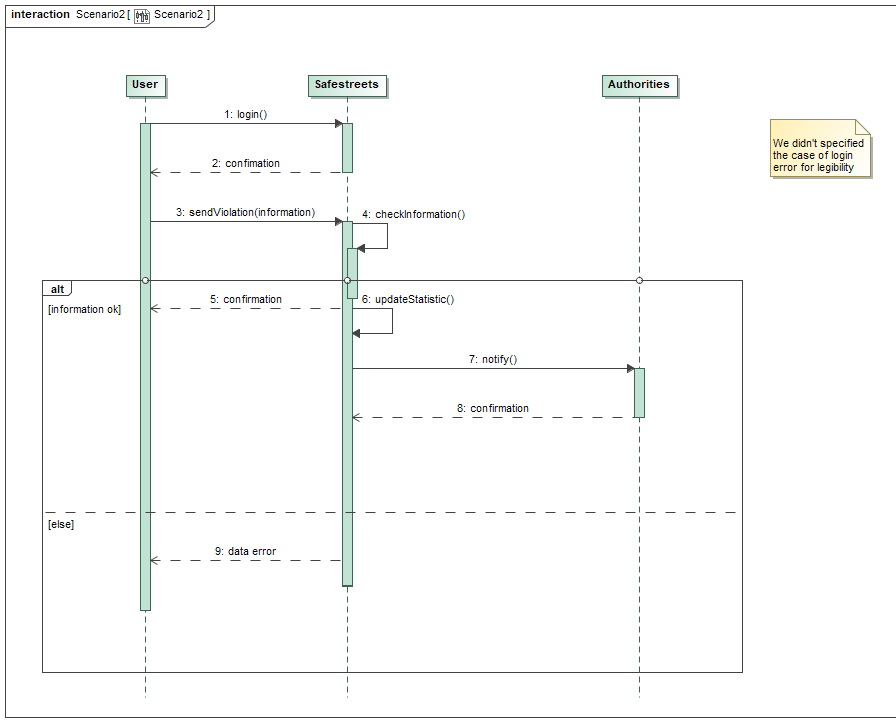
\includegraphics[width=18cm,height=15cm]{Images/SequenceRASD/Scenario2.png}
		\caption{Scenario 2}
	\end{minipage}
\end{figure}
\newpage
\subsubsection{Scenario 5}
\begin{figure}[H]
	\begin{minipage}[b]{0.40\textwidth}
		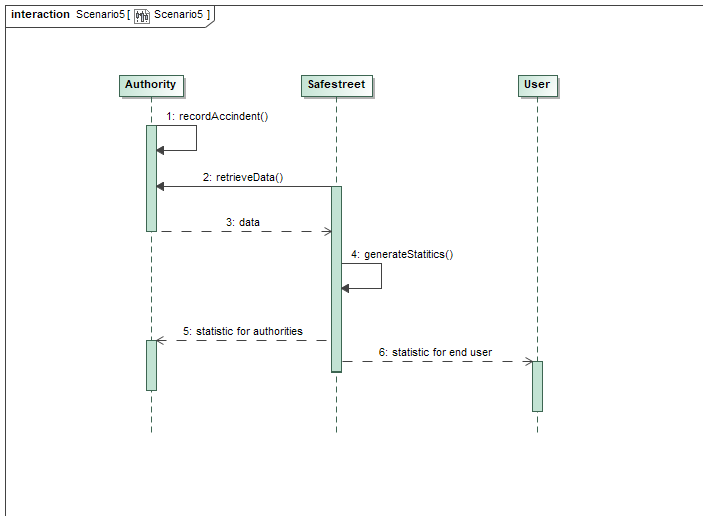
\includegraphics[width=15cm,height=10cm]{Images/SequenceRASD/Scenario5.png}
		\caption{Scenario 5}
	\end{minipage}
\end{figure}
\subsubsection{Scenario 6}
\begin{figure}[H]
	\begin{minipage}[b]{0.40\textwidth}
		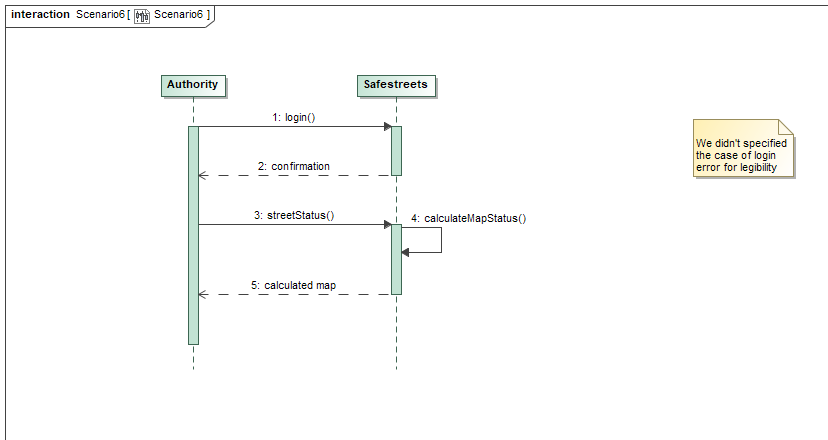
\includegraphics[width=15cm,height=10cm]{Images/SequenceRASD/Scenario6.png}
		\caption{Scenario 6}
	\end{minipage}
\end{figure}

\subsection{Software system attributes}
\subsubsection{Reliability}
The system has to ensure reliability, for this reason we have decided to keep a backup server, updated everyday.
Consistency is guaranteed by the algorithm we have already described.   

\subsubsection{Availability}
The platform has to be available every day, especially in the rush hours because are the ones where there traffic is higher.
 SafeStreets must have an availability of 99\% (3.65 days/year downtime).
 
\subsubsection{Security}
The data have to be encrypted, to grant the privacy (e.g. user's position, car license plate and so forth). 

For this reason is used HTTPS protocol to transmit data from user to SafeStreets.

Every account must have a strong password with the combination of upper-case, lower-case letters and numbers.

\subsubsection{Maintainability}
The system is developed to be compatible with other platform, like the system of the local authority.
There could be maintenance interventions, when it's possible there will be in the hours with the less use of the platform (e.g. midnight).
There will be released updates, both for web-application and system.

\subsubsection{Portability}
The entire system is portable, every user (citizen or local authority) can access to their profile, see data, statistics and make reports of violation from their mobile, their tablet or PCs.

\subsection{Mapping on requirements}
\begin{center}
	\begin{tabular}{ | l | p{2cm} | p{2cm}| p{2cm}|} 
		\hline
		 RawID & GoalID & ReqID & Use Case ID \\
		\hline
		1&G1&RE.1&Scenario 2/3\\
		\hline
		2&G2.1&RE.2&\\
		\hline
		3&G2&RE.3&\\
		\hline
		4&G3.1&RE.4&Scenario 6\\
		\hline
		5&G3&RE.5&\\
		\hline
		6&G4&RE.6&\\
		\hline
		7&G5&RE.7&Scenario 8\\
		\hline
		8&G2&RE.8&\\
		\hline
	\end{tabular}
\end{center}


 